\section{Additional Considerations of Schmidt \textit{et al.} Data Set}
\label{sec:SI_schmidt}
While the data set from \cite{schmidt2016} remains a heroic effort that our
labs continue to return to as a resource, there were steps taken in their
calculation of protein copy number that we argue needed further
consideration. In particular, the authors made an assumption of constant
cellular protein concentration across all growth conditions and used
measurements of cell volume that appear inconsistent with an expected
exponential scaling of cell size with growth rate that is well-documented in
\textit{E. coli} (\cite{schaechter1958, taheriaraghi2015, si2017}).

We begin by looking at their cell volume measurements, which are shown in blue
in Figure \FIG{cell_size_literature}. As a comparison, we also plot cell sizes
reported in three other recent papers: measurements from Taheri-Araghi
\textit{et al.} and Si \textit{et al.} come from the lab of Suckjoon Jun, while
those from Basan \textit{et al.} come  from the lab of Terence Hwa.  Each set of
measurements used microscopy and cell segmentation to determine the length and
width, and then calculated cell size by treating the cell as a cylinder with two
hemispherical ends, as we considered in the previous section. While there is
notable discrepancy between the two research groups, which are both using strain
NCM3722, Basan \textit{et al.} found that this came specifically from
uncertainty in determining the cell width. This is prone to inaccuracy given the
small cell size and optical resolution limits (further described in their
supplemental text). Perhaps the more concerning point is that while each of
these alternative measurements show an exponential increase in  cell size at
faster growth rates, the measurements used by Schmidt \textit{et al.} appear to
plateau. This resulted in an analogous trend in their final reported total
cellular protein per cell as shown in \FIG{schmidt_adjustment_summary}
(purple data points), and is in disagreement with other measurements of total
protein at these growth rates \citep{basan2015}.

\begin{figure}
		\centering{
    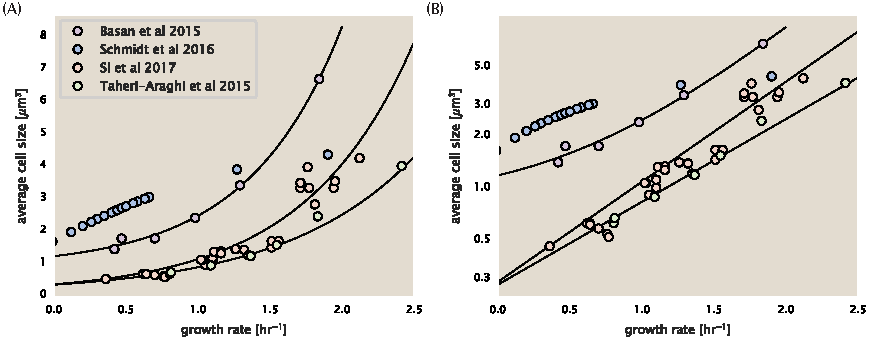
\includegraphics[width=1\textwidth]{SI_figs/figA6_size_data_lit.pdf}
  \caption{\textbf{Measurements of cell size as a function of growth rate.}
	 	(A) Plot of the reported cell sizes from several recent papers.  The data
	 	in blue come from Volkmer and Heinemann, 2011 (\cite{volkmer2011}) and were
	 	used in the work of Schmidt \textit{et al.}. Data from the lab of Terence Hwa
	 	are shown in purple (\cite{basan2015}), while the two data sets shown in green
	 	and light red come from the lab of Suckjoon Jun (\cite{taheriaraghi2015,
	 	si2017}). (B) Same as in (A) but with the data plotted on a logarithmic
	 	y-axis to highlight the exponential scaling that is expected for \textit{E.
	 	coli}.}
  \label{fig:cell_size_literature}
  }
\end{figure}

Since it is not obvious how measurements of cell size influenced their reported
protein abundances, in the following subsections we begin by considering how the
authors determined total protein mass per cell. We then consider three different
approaches to estimate the growth-rate dependent total protein mass and compare
these estimates with those reported by \cite{schmidt2016}. Those results are
summarized in \FIG{cell_size_literature}(B), with the original values from both
\cite{schmidt2016} and \cite{li2014} shown in \FIG{cell_size_literature}(A) for
reference. For most growth conditions, we find reasonable agreement between  our
estimates and the reported total protein per cell. However, for the fastest
growth conditions, with glycerol + supplemented amino acids, and LB media, all
estimates are substantially higher than those originally reported. This is the
main reason why we chose to readjuste protein abundance as shown in
\FIG{total_protein_final}(B) (with the calculation described in section
\nameref{sec:estimate_protein_per_cell}).


\begin{figure}
		\centering
    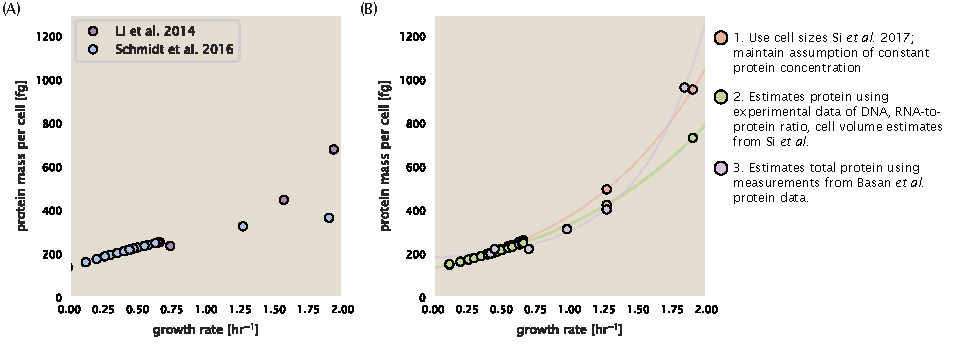
\includegraphics[width=1\textwidth]{SI_figs/figA7_schmidt_protein_corrections.pdf}
  \caption{{\bf Alternative estimates of total cellular protein for the growth conditions
    considered in Schmidt \textit{et al.}} (A) The original protein mass from
    Schmidt \textit{et al.} and Li \textit{et al.} are shown in purple and blue,
    respectively. (B) Three alternative estimates of total protein per cell.
		1.  \textit{light red}: Rescaling of total protein mass assuming a
    growth rate independent protein concentration and cell volumes estimated
    from Si \textit{et al.} 2017. 2. \textit{light green}:  Rescaling of total protein
    mass using estimates of growth rate-dependent protein concentrations and
    cell volumes estimated from Si \textit{et al.} 2017. Total protein per cell
		is calculated by assuming a 1.1 g/ml cellular mass density, 30\% dry mass, with
		90\% of the dry mass corresponding to DNA, RNA, and protein \citep{basan2015}. See
		\nameref{sec:estimate_protein_per_cell} for details on calculation. 3. \textit{light purple}: Rescaling
    of total protein mass using the experimental measurements from Basan
    \textit{et al.} 2015.
	 	}
  \label{fig:schmidt_adjustment_summary}
\end{figure}

\subsection{Effect of cell volume on reported absolute protein abundances}
As noted in \nameref{sec:SI_exp_summary},
the authors from the work in \cite{schmidt2016} calculated proteome-wide protein abundances by first determining
absolute abundances of 41 pre-selected proteins, which relied on adding
synthetic heavy reference peptides into their protein samples at known abundance.  This
absolute quantitation was performed in replicate for each growth condition.
Separately, the authors also performed a more conventional mass spectrometry
measurement for samples from each growth condition, which attempted to maximize
the number of quantified proteins but only provided relative abundances based on
peptide intensities. Finally, using their 41 proteins with absolute abundances
already determined, they then created calibration curves with which to relate
their relative intensity to absolute protein abundance for each growth
condition.  This allowed them to estimate absolute protein abundance for all
proteins detected in their proteome-wide data set. Combined with their flow
cytometry cell counts, they were then able to determine absolute abundance of
each protein detected on a per cell basis.

While this approach provided absolute abundances, another necessary step
to arrive at total cellular protein was to account for any protein loss during
their various protein extraction steps. Here the authors attempted to determine
total protein separately using a BCA protein assay.  In personal communications,
it was noted that determining reasonable total protein abundances by BCA across
their array of growth conditions  was particularly troublesome. Instead, they
noted confidence in their total protein measurements for cells grown in M9
minimal media + glucose and  used this as a reference point with which to
estimate the total protein for all other growth conditions.

For cells grown in M9 minimal media + glucose an average total mass of $M_P$ =
240 fg per cell was measured. Using their reported cell volume, reported as
$V_{orig}$ = 2.84 fl, a cellular protein concentration of $[M_P]_{orig}$ =
$M_P/V_{orig}$ = 85 fg/fl. Now, taking the assumption that cellular protein
concentration is relatively independent of growth rate, they could then estimate
the total protein mass for all other growth conditions from,

\begin{equation}
	M_{P\_i} = [M_P]_{orig} \cdot V_{i}
\end{equation}
where $M_{P_i}$ represents the total protein mass per cell and $V_{i}$ is the
cell volume for each growth condition $i$ as measured in Volkmer and Heinemann,
2011. Here the thinking is that the values of $M_{P_i}$ reflects the total
cellular protein for growth condition $i$, where any discrepancy from their
absolute protein abundance is assumed to be due to protein loss during sample
preparation. The protein abundances from their absolute abundance measurements
noted above were therefore scaled to their estimates and are  shown in Figure
\FIG{schmidt_adjustment_summary} (purple data points).

If we instead consider the cell volumes predicted in the work of Si \textit{et
al.}, we again need to take growth in M9 minimal media + glucose as a reference
with known total mass, but we can follow a similar approach to estimate total
protein mass for all other growth conditions. Letting  $V_{Si\_glu}$ = 0.6 fl be
the predicted cell volume, the cellular protein concentration becomes
$[M_P]_{Si}$ = $M_P/V_{Si\_glu}$ = 400 fg/fl. The new total protein mass per
cell can then be calculated from,

\begin{equation}
	M_{P\_i}' = [M_P]_{Si} \cdot V_{Si\_i}
\end{equation}
where $M_{P_i}'$ is the new protein mass prediction, and $V_{Si_i}$ refers to
the new volume prediction for each condition $i$, These are shown as red data points in
Figure \FIG{schmidt_adjustment_summary}(B).


\subsection{Relaxing assumption of constant protein concentration across growth conditions}
We next relax the assumption that cellular protein concentration is constant and
instead, attempt to  estimate it using experimental data. Here we use the
estimation of total protein mass per cell detailed in
\nameref{sec:estimate_protein_per_cell} for all data points in the
\cite{schmidt2016} data set. The green data points in
\FIG{schmidt_adjustment_summary}(B) show this prediction, and this represents
the approach used to estimate total protein per cell for all data sets.


\subsection{Comparison with total protein measurements from Basan \textit{et al.} 2015.}
One of the challenges in our estimates in the preceding  sections is the need to
estimate protein concentration and cell volumes. These are inherently difficult
to measure accurately due to the small size of \textit{E. coli}. Indeed, for all the
additional measurements of cell volume included in Figure
\FIG{cell_size_literature}, no measurements were performed for cells growing
at rates below 0.5 $hr^{-1}$. It therefore remains to be determined whether our
extrapolated cell volume estimates are appropriate, with the possibility that
the logarithmic scaling of cell size might break down for slower growth.

In our last approach we therefore attempt to estimate total protein using
experimental data that required  no estimates of concentration or cell volume.
Specifically, in the work of  Basan \textit{et al}, the authors measured total
protein per cell for a broad range of growth rates (reproduced in Figure
\FIG{schmidt_adjustment_basan}). These were determined by first measuring
bulk protein from cell lysate, measured by the colorimetric Biuret method
(\cite{You2013}), and then abundance per cell was calculated from cell counts
from either plating cells or a Coulter counter. While it is unclear why Schmidt
\textit{et al.} was unable to take a similar approach, the results from Basan
\textit{et al} appear more consistent with our expectation that cell mass will
increase exponentially with faster growth rates. In addition, although they do
not consider growth rates below about 0.5 $hr^{-1}$, it is interesting to note
that the protein mass per cell appears to plateau to a minimum value at slow
growth. In contrast, our estimates using cell volume so far have predicted that
total protein mass should continue to decrease slightly for slower growing
cells. By fitting this data to an exponential function dependent on growth rate,
we could then estimate the total protein per cell for each growth condition
considered by \cite{schmidt2016}. These are plotted as red data points in
\FIG{schmidt_adjustment_summary}(B).


\begin{figure}
		\centering
    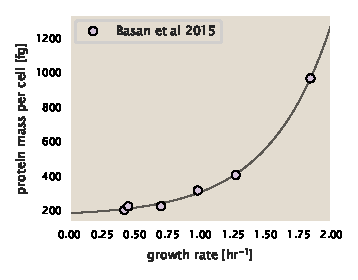
\includegraphics[width=0.5\textwidth]{SI_figs/figA8_schmidt_protein_estimate_basan.pdf}
  \caption{{\bf Total cellular protein reported in Basan \textit{et al.} 2015.}
  Measured protein mass as a function of growth rate as reproduced from Basan
  \textit{et al.} 2015, with cells grown under different levels of nutrient
  limitation. The data was fit to an exponential curve  where protein mass in fg
  per cell is given by 14.65 $e^{2,180 \cdot \lambda}$ + 172 fg per cell, where
  $\lambda$ is the growth rate in hr$^{-1}$).}
  \label{fig:schmidt_adjustment_basan}
\end{figure}
